\chapter{File System II}
\vfill
\section{Block Allocation Strategies}
\subsection{Limitations of Traditional Block Allocation}

Files in modern operating systems typically occupy multiple blocks scattered across a disk. This creates several challenges for efficient file access and management:

\begin{itemize}
  \item \textbf{Linked List Approach:} When blocks are linked together, accessing a file requires traversing all preceding blocks.
    \begin{itemize}
      \item If each block access takes 100 $\mu s$, reading 5 blocks requires 500 $\mu s$.
    \end{itemize}
  
  \item \textbf{File Allocation Table (FAT):} To improve performance, systems often cache the FAT in memory.
    \begin{itemize}
      \item This approach consumes significant memory resources.
      \item For each data block, metadata must be stored in the FAT.
      \item Let's analyze the memory and performance implications for a large file:
    \end{itemize}
\end{itemize}

\begin{center}
\fbox{\begin{minipage}{0.95\textwidth}
  \textbf{Memory and Performance Analysis for FAT}\\[0.5em]
  \textbf{Given:}
  \begin{itemize}
    \item File size: 1 TB ($2^{40}$ bytes)
    \item Block size: 4 KB ($2^{12}$ bytes)
    \item FAT entry size: 4 bytes per block (typical)
    \item Block access time: 100 $\mu$s
  \end{itemize}
  
  \textbf{Number of blocks needed to store the file:}
  \begin{align}
    \text{Blocks} &= \frac{\text{File size}}{\text{Block size}} = \frac{1 \text{ TB}}{4 \text{ KB}} = \frac{2^{40} \text{ bytes}}{2^{12} \text{ bytes}}\\
    &= 2^{40-12} = 2^{28} \text{ blocks}
  \end{align}
  
  \textbf{Memory required for FAT entries (metadata):}
  \begin{align}
    \text{FAT size} &= \text{Number of blocks} \times \text{Entry size}\\
    &= 2^{28} \text{ blocks} \times 4 \text{ bytes/block}\\
    &= 2^{28+2} \text{ bytes} = 2^{30} \text{ bytes} = 1 \text{ GB}
  \end{align}
  
  \textbf{Time to access all metadata (worst case):}
  \begin{align}
    \text{Access time} &= \text{Number of metadata blocks} \times \text{Block access time}\\
    &= \frac{1 \text{ GB}}{4 \text{ KB}} \times 100 \text{ $\mu$s} = \frac{2^{30}}{2^{12}} \times 100 \text{ $\mu$s}\\
    &= 2^{18} \times 100 \text{ $\mu$s} \approx 26.2 \text{ seconds}
  \end{align}
  
  \textbf{Implications:} For a 1 TB file, the FAT approach requires 1 GB of memory just to store metadata. Reading all this metadata would take approximately 26 seconds, making file operations extremely slow.
\end{minipage}}
\end{center}

\begin{center}
  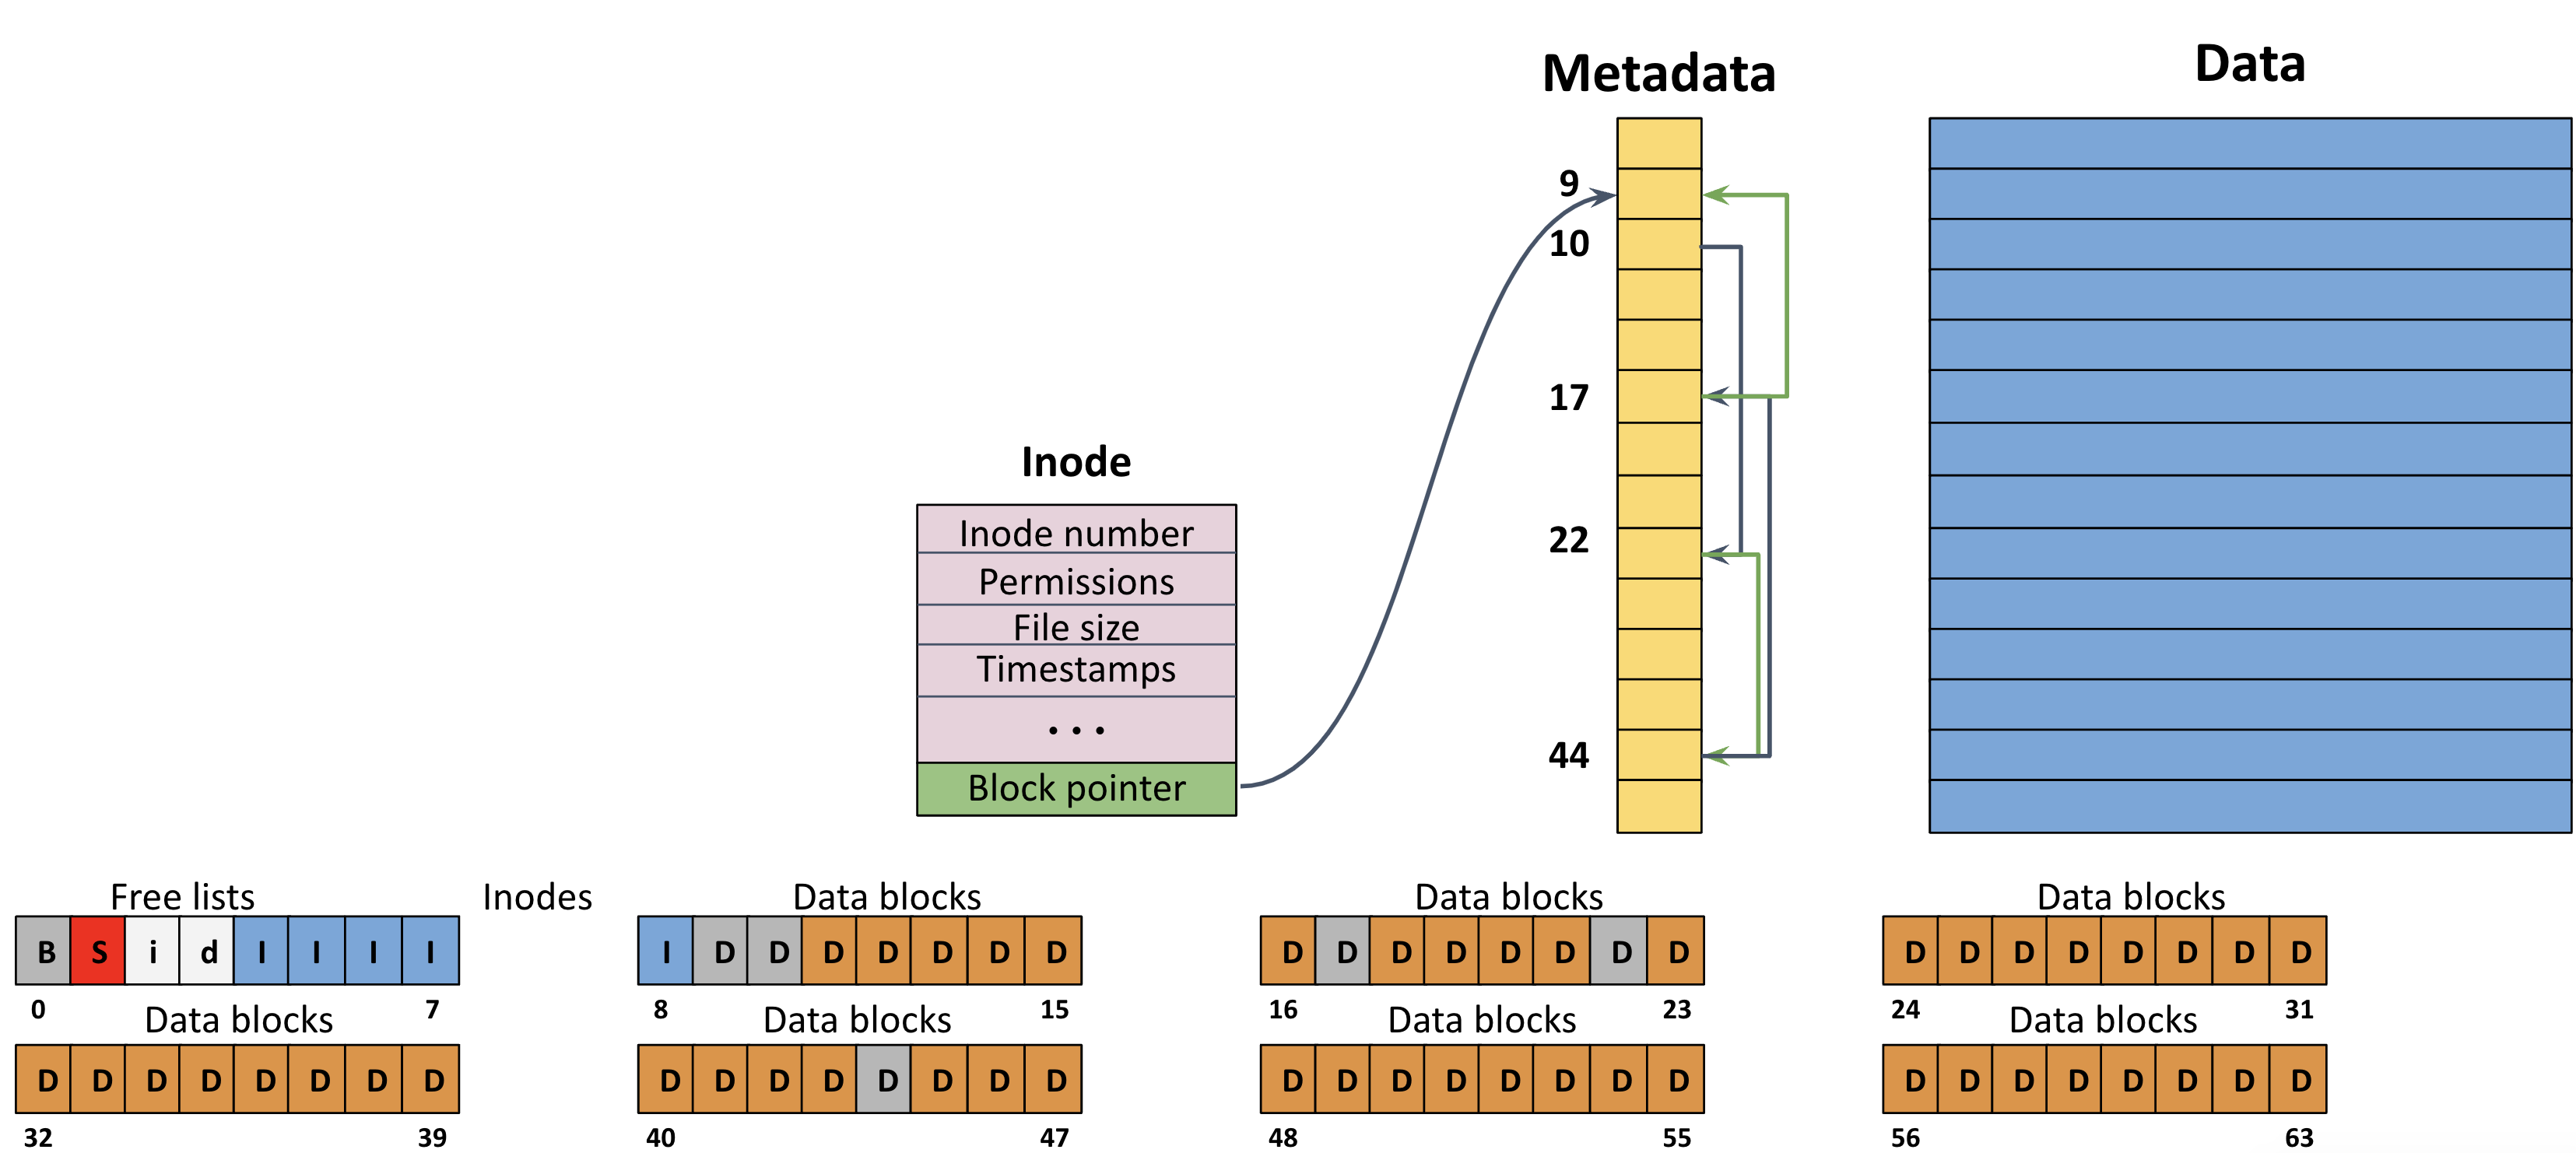
\includegraphics[width=1.05\textwidth]{chapters/L7/images/problem.png}
\end{center}
\newpage
\subsection{Design Goals for Efficient Block Allocation}

A well-designed block allocation strategy should balance several competing requirements:
\begin{itemize}
  \item Minimize memory overhead for metadata
  \item Provide fast access to all parts of a file
  \item Support both small and large files efficiently
  \item Scale gracefully as file size increases
\end{itemize}

\subsection{The Inode Approach}

\noindent
\begin{minipage}{0.55\textwidth}
  \textbf{Key Observation:} File systems must efficiently handle two common types of files:
  
  \begin{enumerate}
    \item \textbf{Small files} ($<$ 50 KB)
      \begin{itemize}
        \item Can be accessed directly with a small set of pointers
        \item Direct inode pointers point to data blocks
      \end{itemize}
    
    \item \textbf{Large files}
      \begin{itemize}
        \item Metadata blocks are allocated as the file grows
        \item Similar to multi-level page tables
        \item Minimizes memory waste through indirection
      \end{itemize}
  \end{enumerate}
\end{minipage}
\hfill
\vline
\hfill
\begin{minipage}{0.35\textwidth}
  \begin{center}
    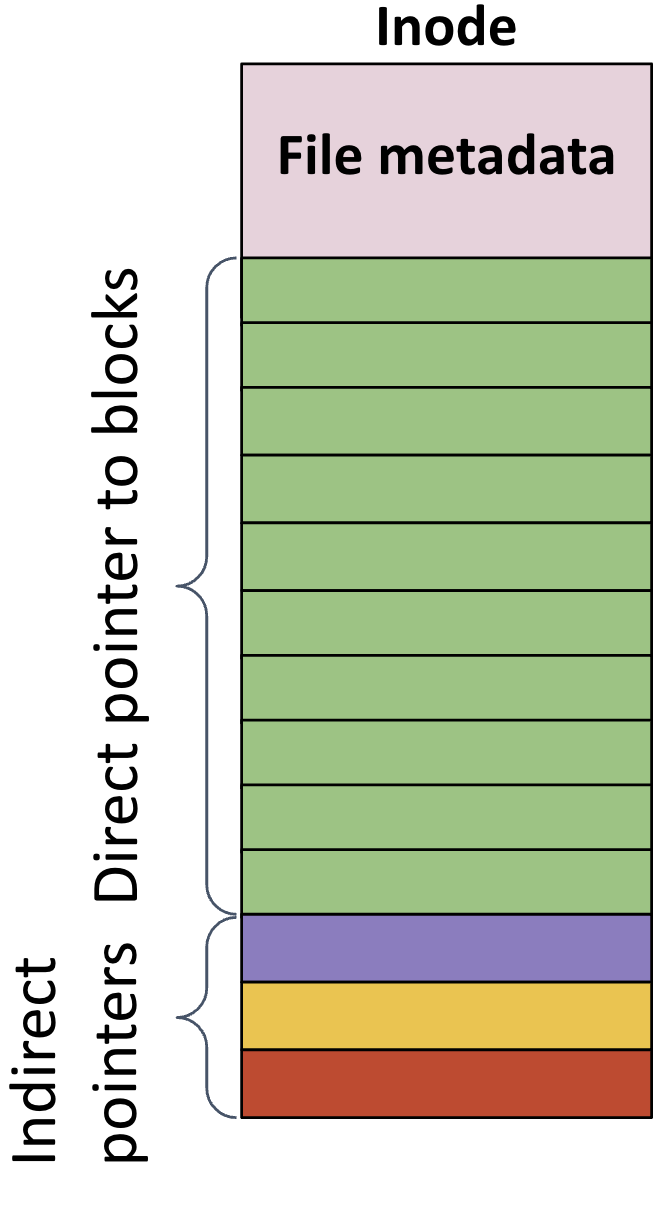
\includegraphics[width=0.85\textwidth]{chapters/L7/images/inode.png}
  \end{center}
\end{minipage}
 
\begin{center}
  \textbf{Inode Pointer Structure}\\[0.5em]
  An inode contains a fixed set of pointers that provide access to data blocks using a hierarchical addressing scheme:
  
  \begin{tabularx}{\textwidth}{|C{0.23\textwidth}|X|C{0.23\textwidth}|}
    \hline
    \textbf{Pointer Type} & \textbf{Description} & \textbf{File Size Range} \\
    \hline
    \textbf{Direct} & 
    First 12 pointers point directly to data blocks, providing immediate, single-step access with no indirection overhead. 
    & Small files ($\leq$ 48 KB) \\
    \hline
    \textbf{Single-Indirect} & 
    Pointer \#13 points to a block of pointers where each entry points to a data block (one level of indirection). 
    & Medium files (up to several MB) \\
    \hline
    \textbf{Double-Indirect} & 
    Pointer \#14 points to a block of pointers; each entry in that block points to another block, which in turn contains pointers to data blocks (two levels of indirection). 
    & Large files (up to several GB) \\
    \hline
    \textbf{Triple-Indirect} & 
    Pointer \#15 points to a block of pointers; each entry points to another block of pointers, then to yet another block before finally reaching data blocks (three levels of indirection). 
    & Very large files (up to TB range) \\
    \hline
    \end{tabularx}
\end{center}

\subsection{Benefits of the Inode Structure}
\begin{itemize}
  \item \textbf{Space Efficiency:} Metadata grows only as needed for larger files
  \item \textbf{Access Speed:} Small files can be accessed with minimal indirection
  \item \textbf{Scalability:} Can address extremely large files with limited overhead
  \item \textbf{Balanced Approach:} Optimizes for both small and large file access patterns
\end{itemize}


\section{File Allocation Approach: Multi-level Indexing}

The multi-level indexing scheme employs a tree-like structure to organize file data blocks, enhancing the efficiency of block retrieval. This approach uses a combination of direct, single indirect, double indirect, and triple indirect pointers to reference data blocks, thereby adapting the indexing depth to the file size.

\subsection*{Key Features and Advantages}

\begin{itemize}
    \item \textbf{Efficient Block Location:} The tree structure allows rapid location of data blocks. Once an indirect block is read, it can reference hundreds of data blocks, making sequential read operations highly efficient.
    
    \item \textbf{Asymmetric Overhead:} The design is asymmetric, meaning that small files benefit from minimal overhead by primarily using direct pointers, while larger files leverage additional levels of indirection without incurring a prohibitive metadata cost.
    
    \item \textbf{Fixed Structure and Simplicity:} The fixed, hierarchical layout simplifies implementation. Metadata is stored separately from data, ensuring there is no conflation between file data and file system metadata.
    
    \item \textbf{No External Fragmentation:} Since data blocks are allocated without external fragmentation, the overall space utilization is improved.
    
    \item \textbf{Performance:} The structure provides reasonable read performance with low seek times, balancing the extra reads required for indirect accesses with the overall efficiency of accessing multiple blocks once an indirect block is in memory.
\end{itemize}

\subsection*{Dynamic Allocation and Practical Considerations}

The allocation dynamics are designed to be adaptive:

\begin{itemize}
    \item \textbf{Small Files:} For a file that contains only a few kilobytes of data, direct pointers are used. For example, reading a 4~KB block from a file accessed via a direct pointer incurs minimal overhead.
    
    \item \textbf{Large Files:} As the file size grows, additional levels of indexing are activated. With a three-level (triple indirect) indexing, even a file requiring 16~KB of data can be managed efficiently. The extra levels allow the file system to scale, enabling support for very large files without a linear increase in metadata.
    
    \item \textbf{Mixed Access Patterns:} The tree-like indexing provides a good balance between random access (via direct pointers) and sequential reads (via high-degree indirect blocks), which is beneficial for different file access patterns.
\end{itemize}

\begin{center}
  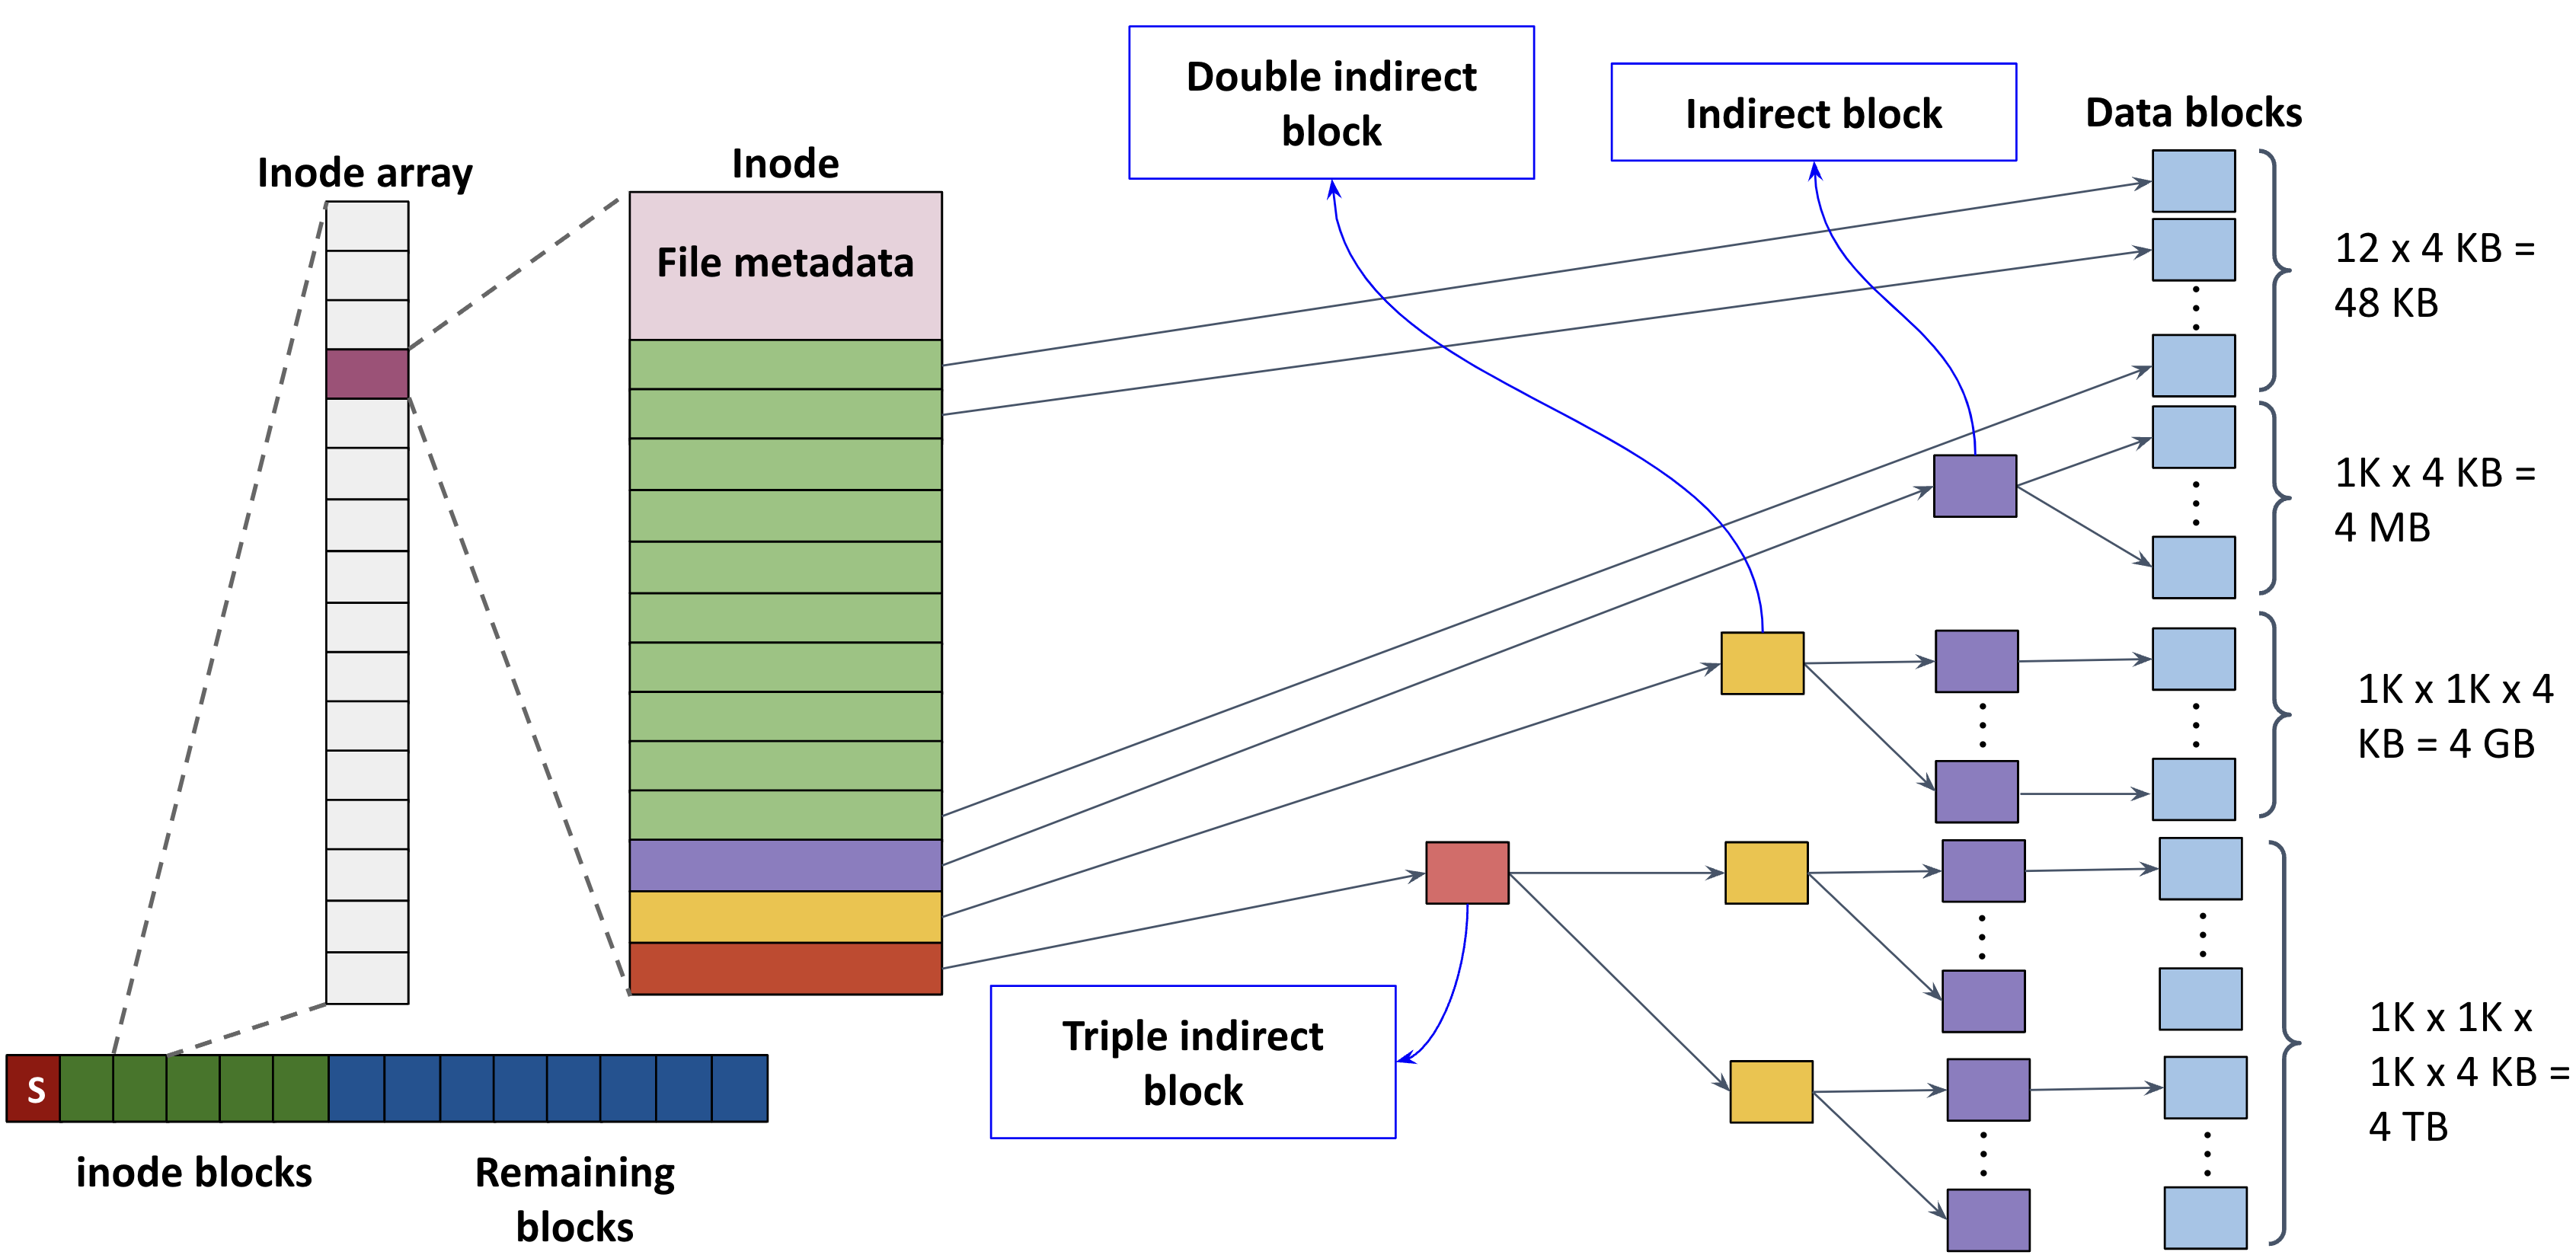
\includegraphics[width=0.8\textwidth]{chapters/L7/images/multi.png}
\end{center}
The multi-level indexing file allocation method enhances both performance and scalability by adapting the index structure to the file size, ensuring low overhead for small files while supporting efficient access for large files.
